
%\documentclass[12pt,draft]{article}
\documentclass[12pt]{article}


\usepackage[english]{babel}
%\usepackage[frenchb]{babel}
\usepackage{CJK}
\usepackage{mathrsfs}
\usepackage{amsmath,amsthm,amsfonts,amssymb}
\usepackage{geometry}
\usepackage{fancyhdr}
\usepackage{indentfirst}
\usepackage{float}
\usepackage[dvips]{graphicx}
\usepackage{subfigure}
\usepackage[font=small]{caption}
\usepackage{threeparttable}
\usepackage{cases}
\usepackage{multicol}
\usepackage{url}
\usepackage{amsmath}
\usepackage{bm}
\usepackage{xcolor}
\usepackage{overpic}
\usepackage{natbib}
\usepackage[utf8]{inputenc}

\usepackage{natbib}
\usepackage{graphicx}
\usepackage{hyperref}
\usepackage{verbatim}
\numberwithin{equation}{section}
\usepackage{titlesec}
\setcounter{secnumdepth}{4}
\titleformat{\paragraph}
{\normalfont\normalsize\bfseries}{\theparagraph}{1em}{}
\titlespacing*{\paragraph}
{0pt}{3.25ex plus 1ex minus .2ex}{1.5ex plus .2ex}

\geometry{left=1.5cm,right=1.5cm,top=1.5cm,bottom=1.5cm}
\setlength{\parskip}{0.3\baselineskip}
\setlength{\headheight}{15pt}
\begin{document}\small
  \renewcommand\figurename{Fig.}
  %\renewcommand\arraystretch{1.0}
    \title{Probalistic Graphic Model\cite{Coursera}\cite{koller2009probabilistic} Notes}
    \author{Yan JIN}
    \pagestyle{fancy}\fancyhf{}
    \lhead{}\rhead{JIN Yan}
    \lfoot{\textit{}}\cfoot{}\rfoot{\thepage}
    \renewcommand{\headrulewidth}{1.pt}
    \renewcommand{\footrulewidth}{1.pt}
  \maketitle
  
\tableofcontents
\newpage

\section{Representation}
\subsection{Introduction and Overview}
Model: The model is a \textbf{declarative representation} of our understanding of the world. It's \textbf{declarative} means that the representation stands on its own, which means that we can look into it and make sense of it \textbf{aside from any algorithm} that we might choose to apply on. 

\begin{enumerate}
	\item Representation
	
	- Directed and undirected
	
	- Temperal and plate models
	\item Inference
	
	- Exact and approximate
	
	- Decision making
	\item Learning
	
	- Parameters and structure
	
	- With and without complete data
\end{enumerate}

\subsubsection{Distributions (Chapters 2.1.1 to 2.1.3)}

\subsubsection{Factors (Chapter 4.2.1)}

\begin{comment}

\end{comment}

\subsubsection{Quiz}
\begin{figure}[H]
  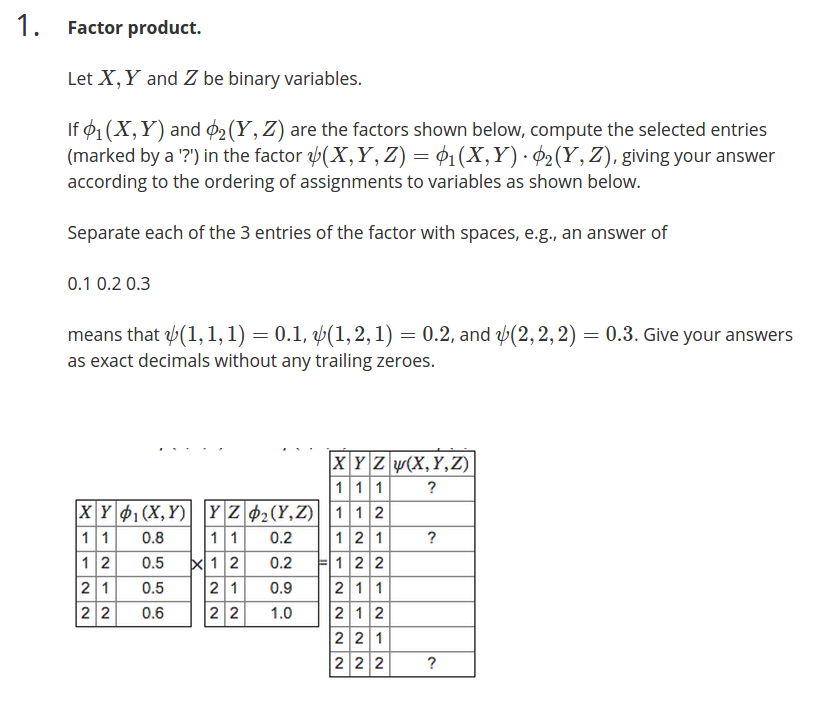
\includegraphics[width=\linewidth]{PGMpics/01-01-01.png}
  \caption{Exercise 01-01-01}
  \label{fig:01-01-01}
\end{figure}

\begin{figure}[H]
  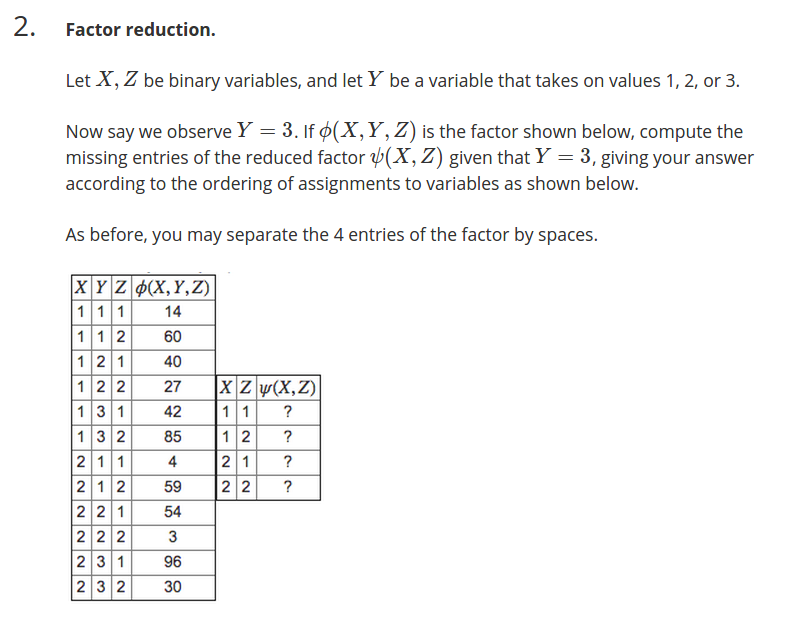
\includegraphics[width=\linewidth]{PGMpics/01-01-02.png}
  \caption{Exercise 01-01-02}
  \label{fig:01-01-02}
\end{figure}

\begin{figure}[H]
  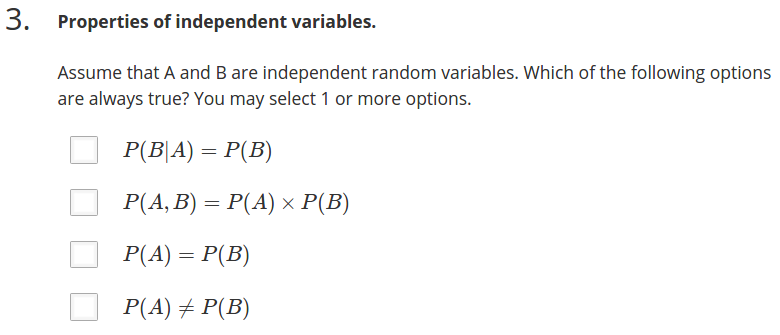
\includegraphics[width=\linewidth]{PGMpics/01-01-03.png}
  \caption{Exercise 01-01-03}
  \label{fig:01-01-03}
\end{figure}

\begin{figure}[H]
  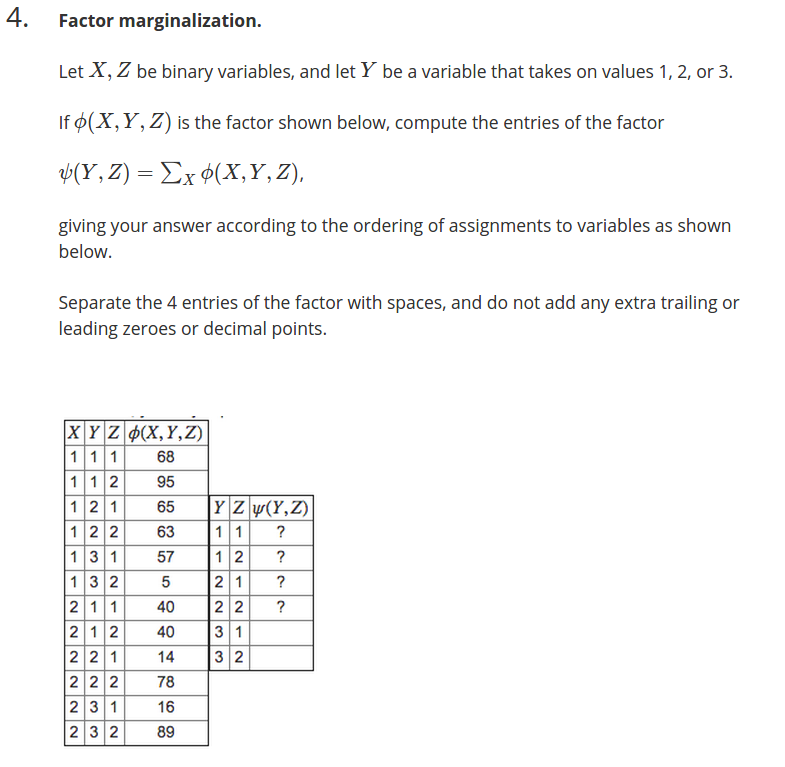
\includegraphics[width=\linewidth]{PGMpics/01-01-04.png}
  \caption{Exercise 01-01-04}
  \label{fig:01-01-04}
\end{figure}

\subsubsection{Answers}
01-01-01: 0.16 0.45 0.6;

01-01-02: 42 85 96 30;

01-01-03: Choose 1st and 2nd items;

01-01-04: 108 135 79 141;

\subsection{Baysian Network (Directed Models)}
\subsubsection{Semantics and Factorization (Chapters 3.2.1, 3.2.2)}
If you are unfamiliar with genetic inheritance, please watch this short \href{https://www.khanacademy.org/science/biology/classical-genetics/mendelian--genetics/v/introduction-to-heredity}{Khan Academy video} for some background.

CPD: Conditional Probability Distribution;

DAG: Directed Acyclic Graph;

P \textbf{factorizes} over Graph G if:
$P(X_1,...,X_n)=\prod_i\ P(X_i|Par_G(X_i))$
\subsubsection{Reasoning Patterns (Chapter 3.2.1.2)}
Causal Reasoning(Father to Son), Evidential Reasoning(Son to Father), Intercausal Reasoning;
\subsubsection{Flow of Probabilistic Influence (Chapter 3.3.1)}
When influence can flow from X to Y via Z, we can say that the trail $X \rightleftharpoons Z \rightleftharpoons Y$ is \textbf{active};

v-structure;

(Definition 3.6) Let $\mathcal{G}$ be a BN structure, and $X_1 \rightleftharpoons ... \rightleftharpoons X_n$ a trail in $\mathcal{G}$. Let $\mathbf{Z}$ be a subset of observed variables. The trail $X_1 \rightleftharpoons ... \rightleftharpoons X_n$ \textbf{is active given} $\mathbf{Z}$ if:
\begin{itemize}
	\item Whenever we have a v-structure $X_{i-1} \rightarrow X_i \leftarrow X_{i+1}$, then $X_i$ or one of its descendants are in $\mathbf{Z}$;
	\item No other node along the trail is in $\mathbf{Z}$;
\end{itemize}

\subsubsection{Quiz}
\begin{figure}[H]
	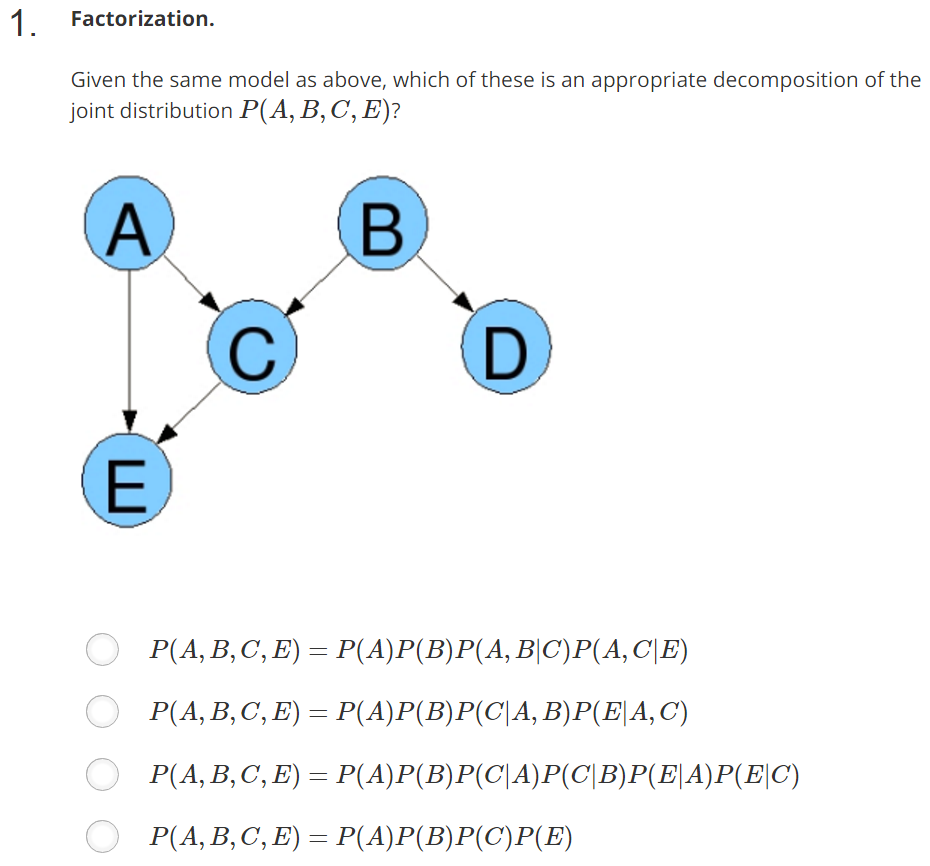
\includegraphics[width=\linewidth]{PGMpics/01-02-01.png}
	\caption{Exercise 01-02-01}
	\label{fig:01-02-01}
\end{figure}
\begin{figure}[H]
	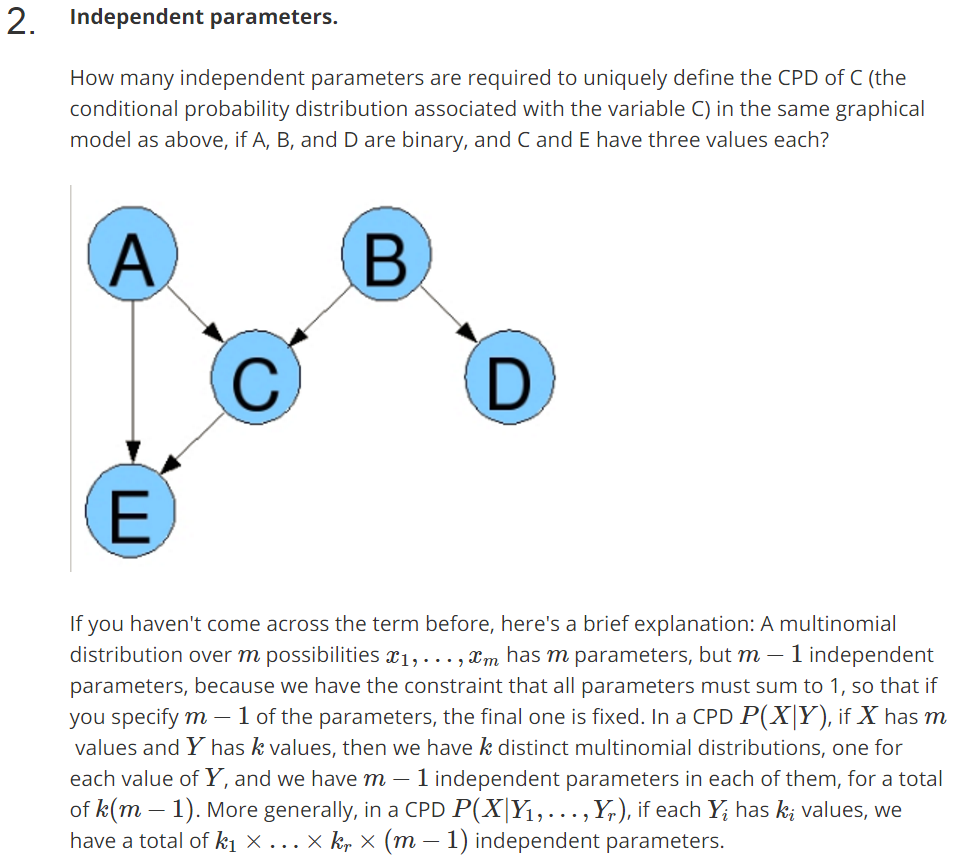
\includegraphics[width=\linewidth]{PGMpics/01-02-02-1.png}
	%\caption{Exercise 01-02-02-01}
	\label{fig:01-02-02-1}
\end{figure}
\begin{figure}[H]
	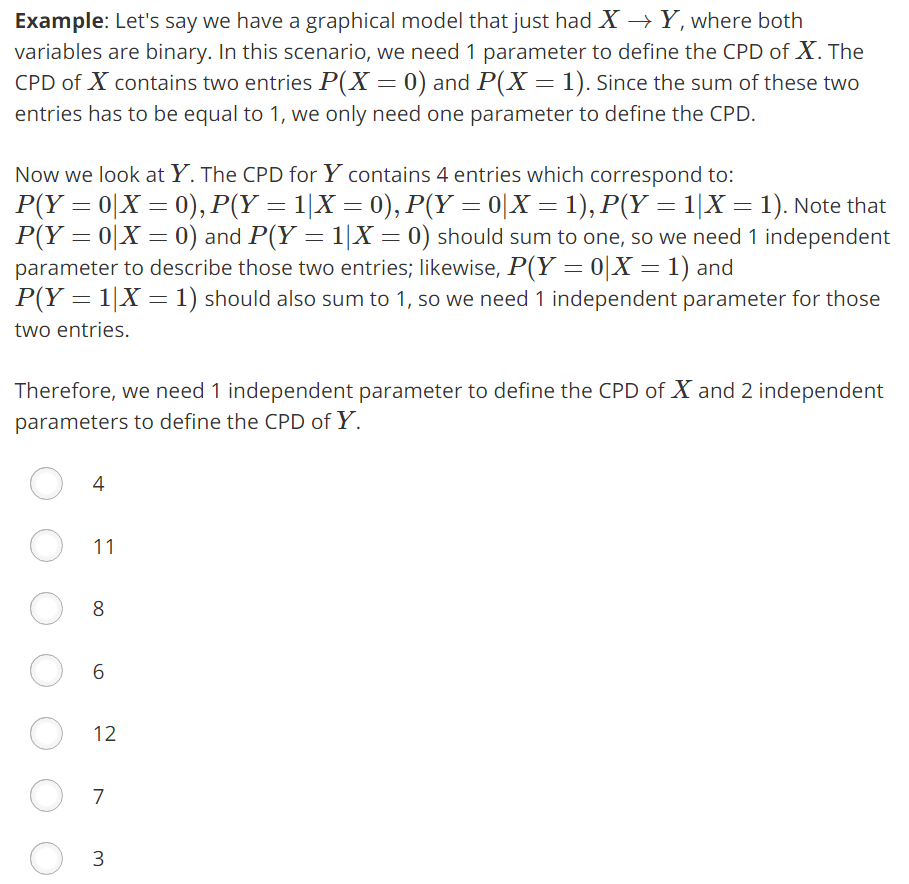
\includegraphics[width=\linewidth]{PGMpics/01-02-02-2.png}
	\caption{Exercise 01-02-02}
	\label{fig:01-02-02-2}
\end{figure}
\begin{figure}[H]
	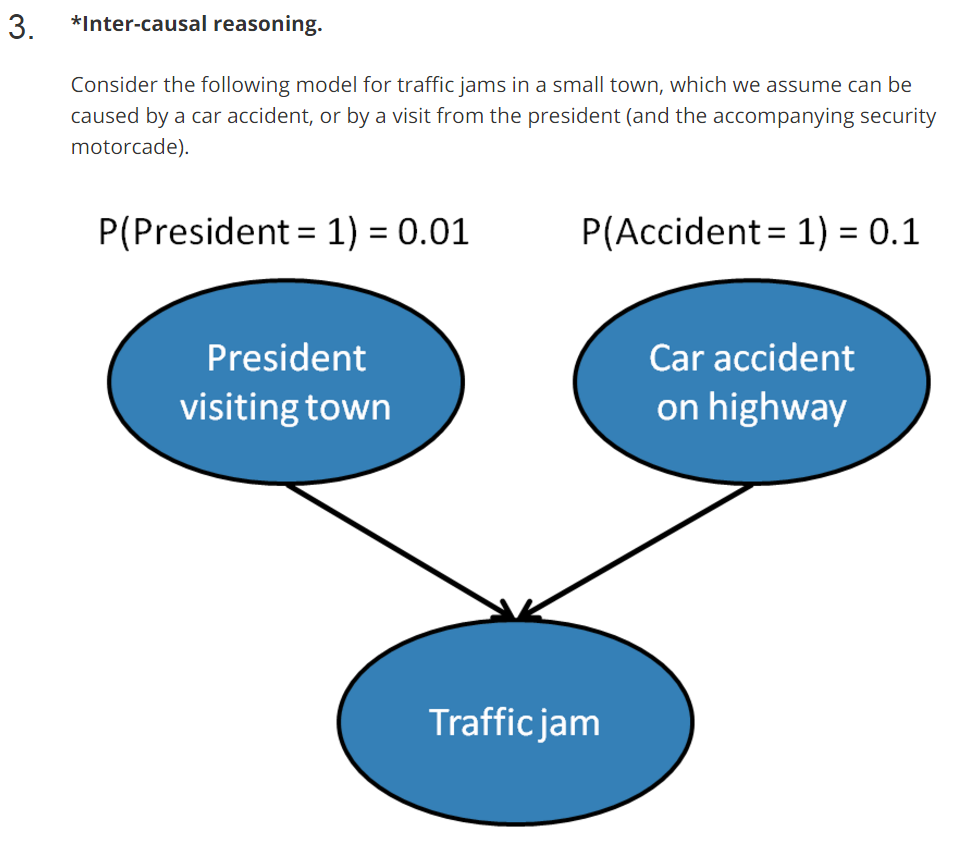
\includegraphics[width=\linewidth]{PGMpics/01-02-03-1.png}
	%\caption{Exercise 01-02-03-01}
	\label{fig:01-02-03-1}
\end{figure}
\begin{figure}[H]
	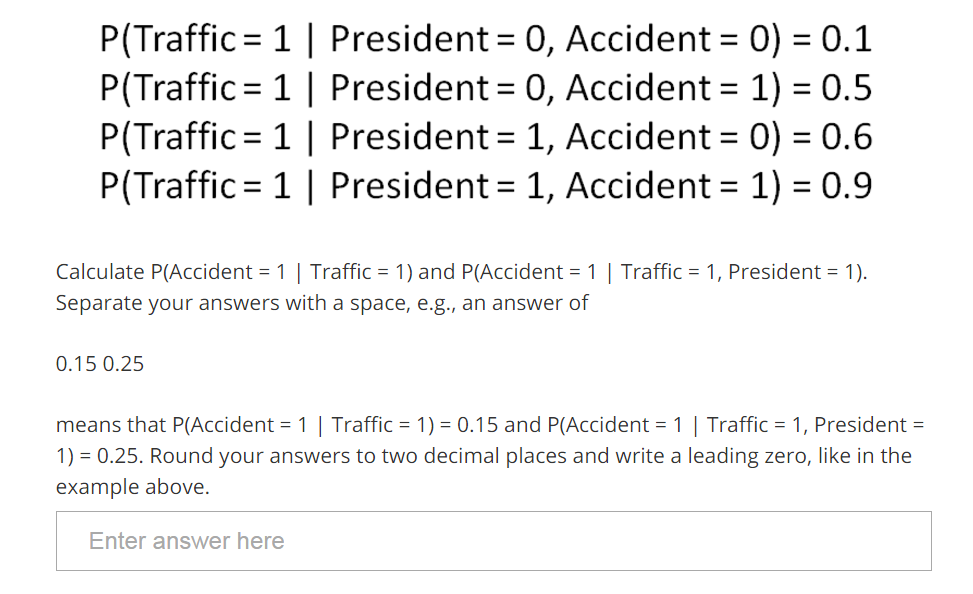
\includegraphics[width=\linewidth]{PGMpics/01-02-03-2.png}
	\caption{Exercise 01-02-03}
	\label{fig:01-02-03-2}
\end{figure}

\subsubsection{Answers}
01-02-01: Choose 2nd item;

01-02-02: (3-1)*2*2 = 8;

01-02-03: 0.34 0.14;
\begin{align*}
P(A=1|T=1)&=\frac{P(A=1,T=1)}{P(T=1)}
\\ &=\frac{P(A=1,T=1,P=0)+P(A=1,T=1,P=1)}{P(T=1)}
\\ &=\frac{0.1*0.99*0.5+0.9*0.1*0.01}{0.1*0.99*0.5+0.9*0.1*0.01+0.1*0.99*0.9+0.6*0.01*0.9}=0.34 \\
P(A=1|T=1,P=1)&=\frac{P(A=1,T=1,P=1)}{P(T=1,P=1)}
\\ &=\frac{P(A=1,T=1,P=1)}{P(A=0,T=1,P=1)+P(A=1,T=1,P=1)}
\\ &=\frac{P(P=1)P(A=1)P(T=1|A=1,P=1)}{P(P=1)P(A=0)P(T=1|A=0,P=1)+P(P=1)P(A=1)P(T=1|A=1,P=1)}
\\ &= \frac{0.01*0.1*0.9}{0.01*0.9*0.6+0.01*0.1*0.9} = 0.14
\end{align*}

\subsubsection{Conditional Independence (Chapters 2.1.4, 3.1)}
\subsubsection{Independencies in Bayesian Networks (Chapter 3.3.1)}
(Definition 3.7) Let $\mathbf{X}$,$\mathbf{Y}$,$\mathbf{Z}$ be three set of nodes in $\mathcal{G}$. X and Y are \textbf{d-separated} give $\mathbf{Z}$, if there is no active trail between andy node $X\in\mathbf{X}$ and $Y\in\mathbf{Y}$ given $\mathbf{Z}$.

Theorem: If P factorizes over G, and d-$sep_{G}
(\mathbf{X},\mathbf{Y}|\mathbf{Z}$) then P satisfies ($\mathbf{X} \bot \mathbf{Y} | \mathbf{Z}$);

Any node is d-separated from its non-descendants given its parents;
Then from the theorem above, we have:
If P factorizes over G, then in P, any variable is independent of its non-descendants given its parents.

Definition: If P satisfies I(G), then G is an \textbf{I-map}(independency map) of P; where
\[I(G)=\{(\mathbf{X} \bot \mathbf{Y} | \mathbf{Z}):d\text{-}sep_{G}
	(\mathbf{X},\mathbf{Y}|\mathbf{Z})\} \]

Factorization $\Rightarrow$ Independence:

Theorem: If P factorizes over G, then G is an I-map for P;

Independence $\Rightarrow$ Factorization:

Theorem: If G is an I-map for P, then P factorizes over G;

\textbf{Summary:} 

Two equivalent views of graph structure:
\begin{itemize}
	\item Factorization: G allows P to be represented;
	\item I-map: Independencies encoded by G hold in P;
\end{itemize}

\subsubsection{Naive Bayes (Chapter 3.1.3)}
\begin{figure}[H]
	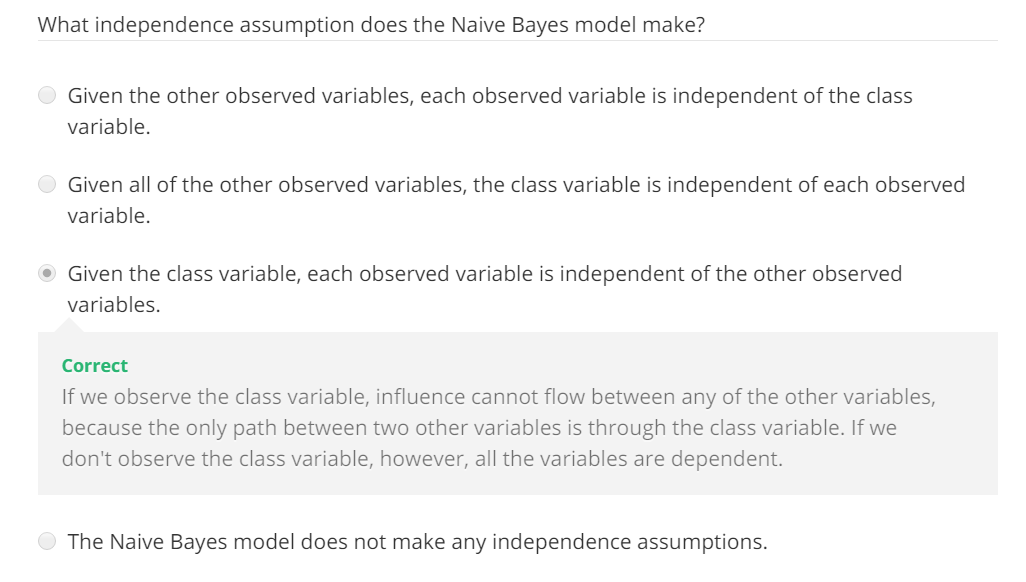
\includegraphics[width=\linewidth]{PGMpics/NaiveBayes.png}
	\caption{Naive Bayes Assumption}
	\label{fig:NaiveBayes}
\end{figure}

\subsubsection{Quiz}
\begin{figure}[H]
	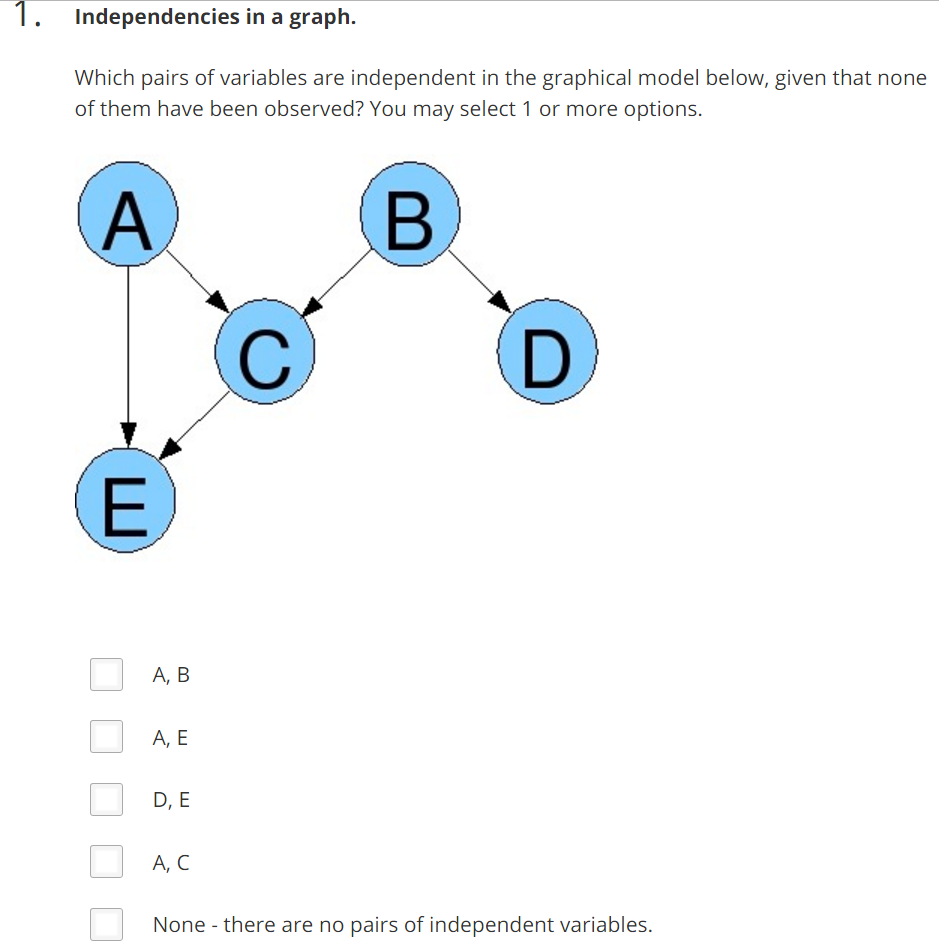
\includegraphics[width=\linewidth]{PGMpics/01-03-01.png}
	\caption{Exercise 01-03-01}
	\label{fig:01-03-01}
\end{figure}
\begin{figure}[H]
	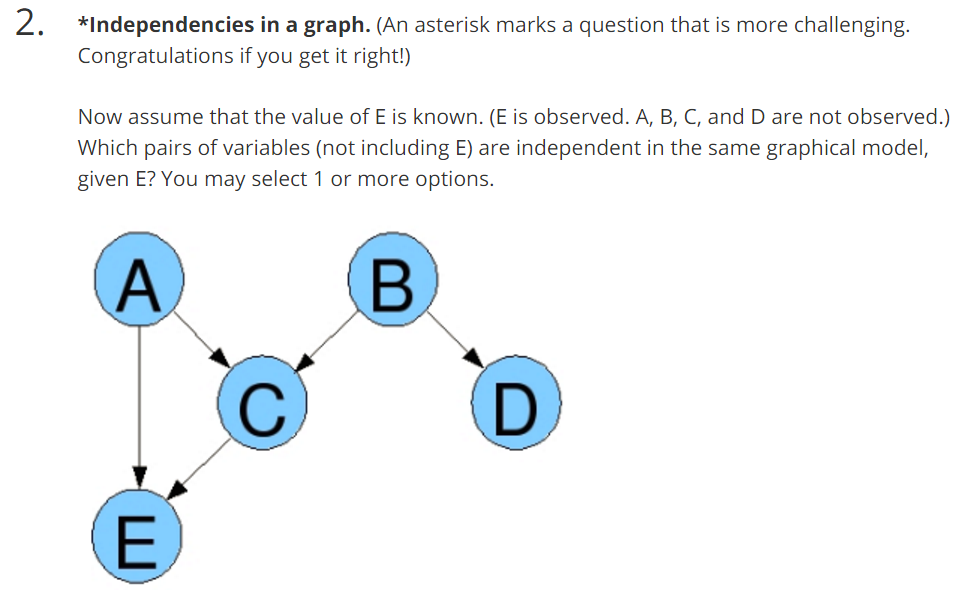
\includegraphics[width=\linewidth]{PGMpics/01-03-02-1.png}
	%\caption{Exercise 01-03-02-01}
	\label{fig:01-03-02-1}
\end{figure}
\begin{figure}[H]
	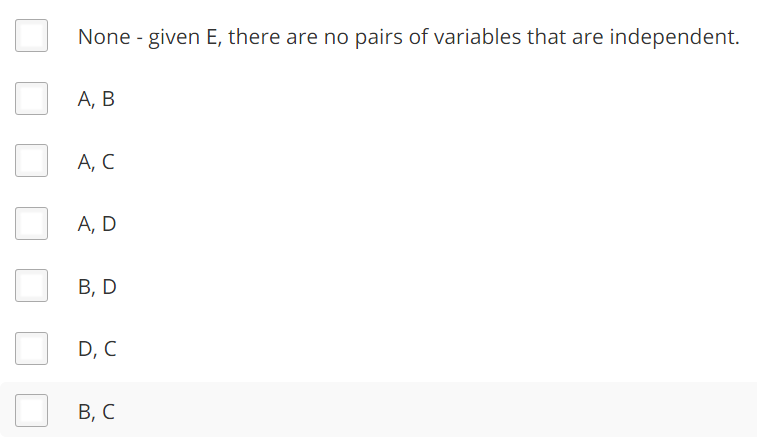
\includegraphics[width=\linewidth]{PGMpics/01-03-02-2.png}
	\caption{Exercise 01-03-02}
	\label{fig:01-03-02-2}
\end{figure}
\begin{figure}[H]
	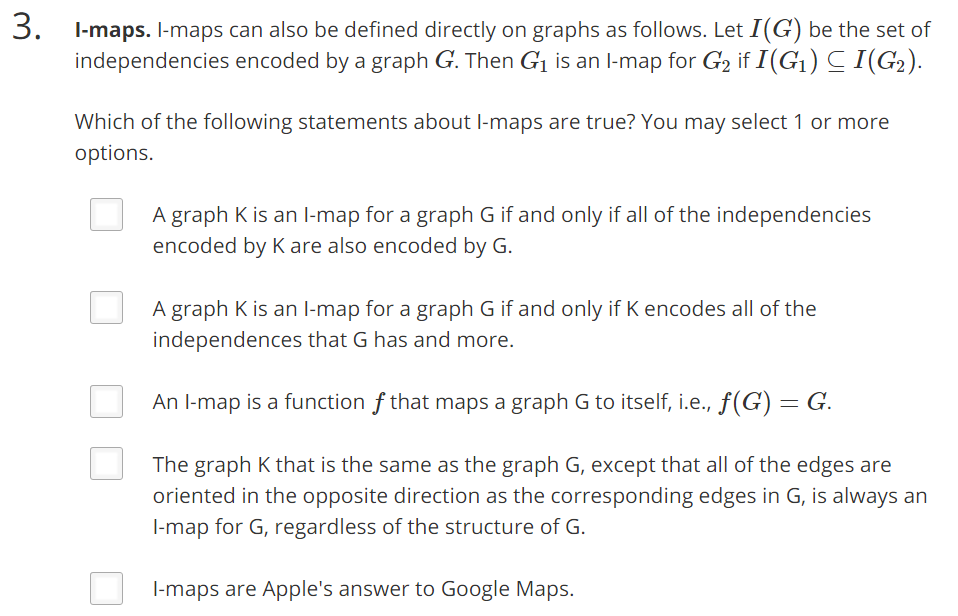
\includegraphics[width=\linewidth]{PGMpics/01-03-03.png}
	\caption{Exercise 01-03-03}
	\label{fig:01-03-03}
\end{figure}
\begin{figure}[H]
	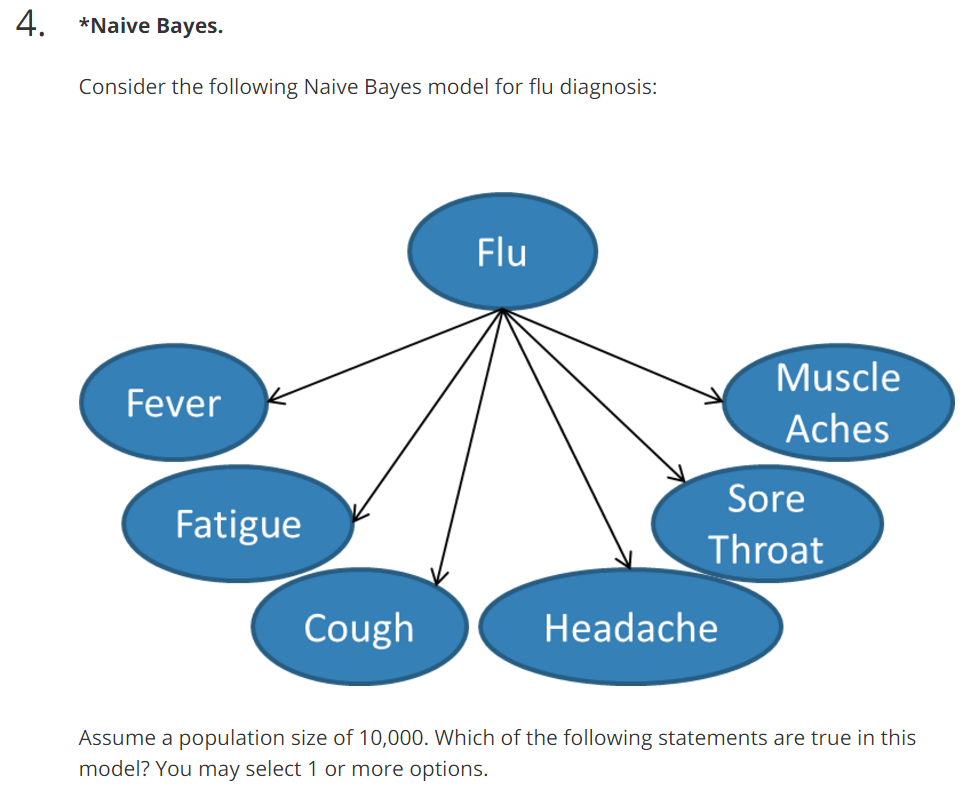
\includegraphics[width=\linewidth]{PGMpics/01-03-04-1.png}
	%\caption{Exercise 01-03-04-01}
	\label{fig:01-03-04-1}
\end{figure}
\begin{figure}[H]
	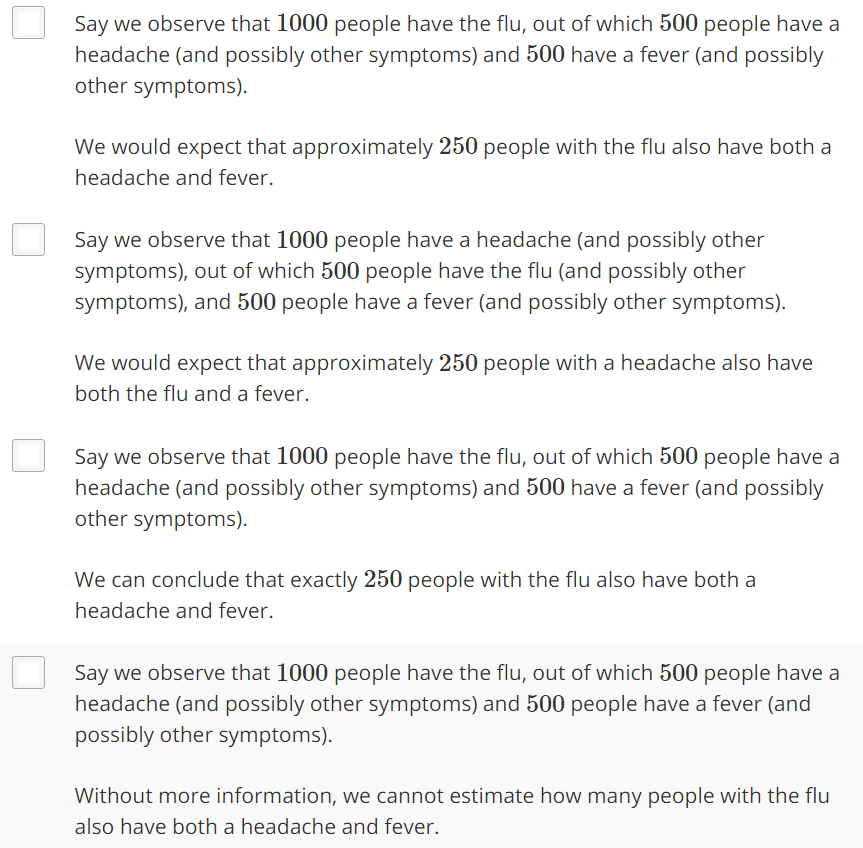
\includegraphics[width=\linewidth]{PGMpics/01-03-04-2.png}
	\caption{Exercise 01-03-04}
	\label{fig:01-03-04-2}
\end{figure}
\begin{figure}[H]
	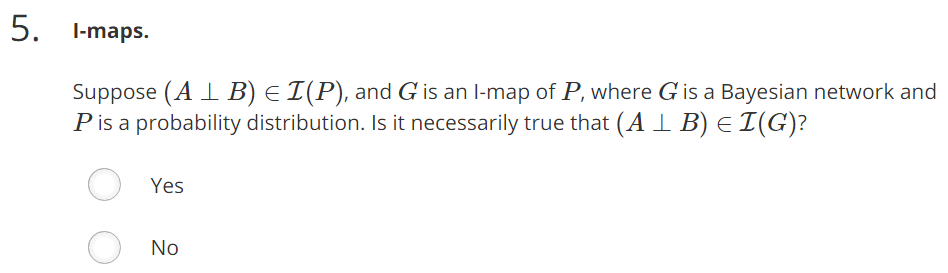
\includegraphics[width=\linewidth]{PGMpics/01-03-05.png}
	\caption{Exercise 01-03-05}
	\label{fig:01-03-05}
\end{figure}
\subsubsection{Answers}
01-03-01: Choose 1st item; 

D,E: There is an active trail connecting D and E that goes through B and C; 

01-03-02: Choose 1st item;

A,D: Observing E activates the V-structures around C and E. Hence, influence can flow from A to B through C, and therefore from A to D through C and B.

D,C: Influence can flow along the active trail $D \leftarrow B \rightarrow C$.

01-03-03: Choose 1st item;

For the 4th item: This is not always true; consider the V-structure $A \rightarrow B \leftarrow C$.

01-03-04: Choose 1st item;
\[ P(Headache=1,Fever=1|Flu=1)=P(Headache=1|Flu=1) \times P(Fever=1|Flu=1)\]

01-03-05: Choose No;

Since G is an I-map of P, all independencies in G are also in P. However, this doesn't mean that all independencies in P are also in G. An easy way to remember this is that \textbf{the complete graph}, which has no independencies, \textbf{is an I-map of all distributions}.

\subsubsection{Bayesian Networks: Knowledge Engineering}
\paragraph{Application - Medical Diagnosis Chapter 3.2: Box 3.D (p. 67)}

\subsection{Template Models for Bayesian Networks}
\subsubsection{Overview (Chapter 6.1)}
\textbf{Template Variables} is instantiated(duplicated) multiple times;

\textbf{Template Models} is a Language that tell us how template variables can be the dependency models from template.
\begin{figure}[H]
	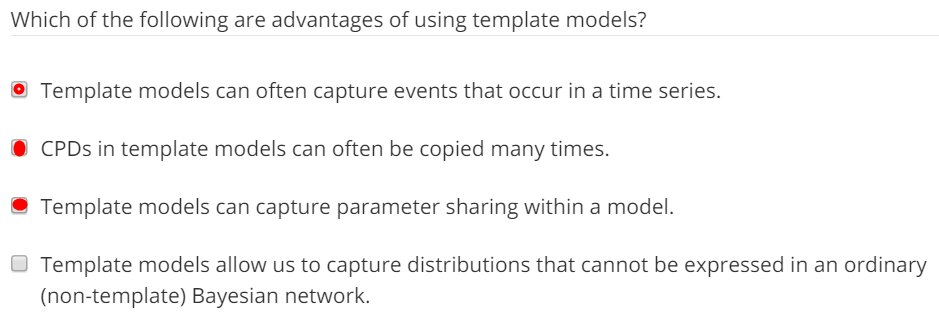
\includegraphics[width=\linewidth]{PGMpics/TemplateModels.png}
	\caption{Template Models}
	\label{fig:TemplateModels}
\end{figure}
Template models are a convenient way of representing Bayesian networks that have a high amount of parameter sharing and structure. However, they are merely compact representations of a fully unrolled Bayesian network, thus have no additional representative powers.
\begin{itemize}
	\item Temperal Models: for dealing with temporal processes, for example, where we have replication over time.
	\begin{itemize}
		\item Dynamic Bayesian networks (DBN); Hidden Markov Models (HMM);
	\end{itemize}
	\item Object relation models:
	\begin{itemize}
		\item Directed Models: Plate models;
		\item Undirected Models;
	\end{itemize}
\end{itemize}

\subsubsection{Temporal Models - DBNs (Chapters 6.2, 6.3)}
Markov Assumption;

Time Invariance, so we can replicated the \textbf{Template probability model} for ALL t;

2-time-slice Bayesian Network (2TBN);

Dynamic Bayesian Network (DBN);
\subsubsection{Temporal Models - HMMs (Chapters 6.2, 6.3)}
Applications:
\begin{itemize}
	\item Robot localization
	\item Speech recognition
	\item Biological sequence analysis
	\item Text annotation
\end{itemize}
\subsubsection{Plate Models (Chapters 6.4.1)}

\subsection{Structured CPDs for Bayesian Networks}
\subsubsection{Overview (Chapter 5.1, 5.2)}
\begin{figure}[H]
	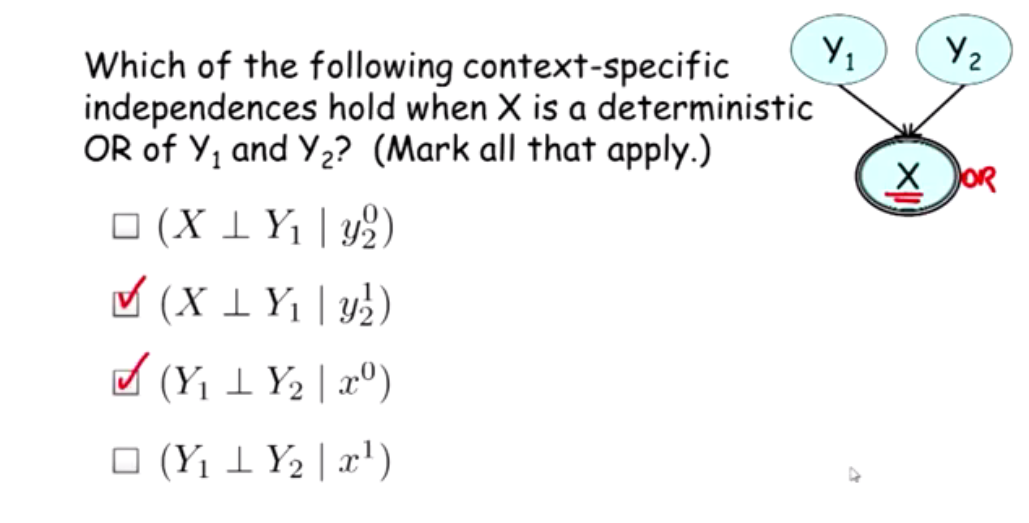
\includegraphics[width=\linewidth]{PGMpics/OverviewStructuredCPD.png}
	\caption{An example of Context-Specific Independence}
	\label{fig:OverviewStructuredCPD}
\end{figure}
\subsubsection{Tree-Structured CPDs (Chapter 5.3)}
\begin{figure}[H]
	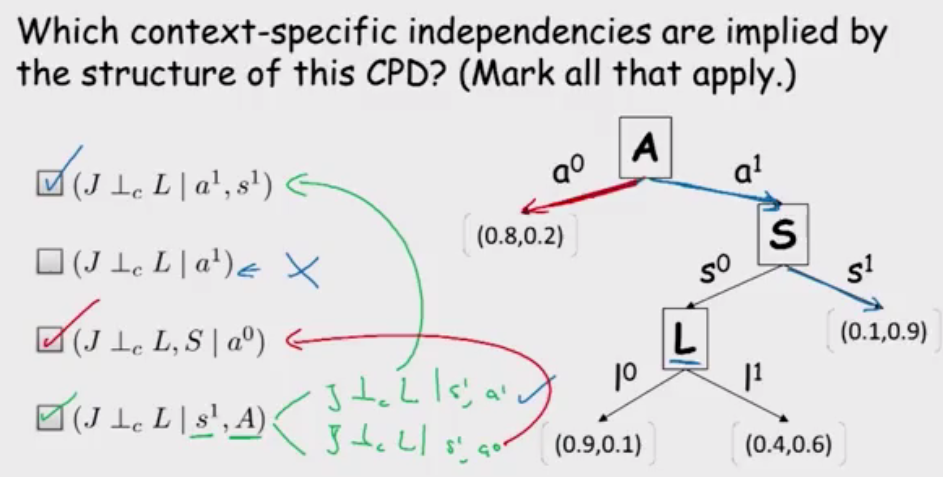
\includegraphics[width=\linewidth]{PGMpics/TreeStructuredCPDs.png}
	\caption{An example of Context-Specific Independence for Tree Structured CPDs}
	\label{fig:TreeStructuredCPDs}
\end{figure}
\subsubsection{Independence of Causal Influence (Chapter 5.4)}
\subsubsection{Continuous Variables (Chapter 5.5)}
Linear Gaussian;

Conditional Linear Gaussian;

Nonlinear Gaussian - Robot Localization, Robot Motion Model;

\subsection{Markov Network (Undirected Models)}
\subsubsection{Pairwise Markov Networks (Chapter 4.1)}









\subsubsection{General Gibbs Distribution (Chapter 4.2.2)}
\subsubsection{Conditional Random Fields (Chapter 4.6.1)}
\subsubsection{Independencies in Markov Networks (Chapter 4.3.1)}
\subsubsection{I-Maps and Perfect Maps (Chapter 3.3.4)}
\subsubsection{Local Structure in Markov Networks}
\subsubsection{Log-Linear Models (Chapter 4.4, p. 125)}
\subsubsection{Shared Features in Log-Linear Models (Chapter 4: Box 4.B (p. 112), Box 4.C (p. 126), Box 4.D (p. 127))}

\subsection{Decision Making}
\subsubsection{Maximum Expected Utility (Chapter 22.1.1, 23.2.104, 23.4.1-2, 23.5.1)}
\subsubsection{Utility Functions (Chapter 22.2.1-3, 22.3.2, 22.4.2)}
\subsubsection{Value of Perfect Information (Chapter 23.7.1-2)}

\subsection{Knowledge Engineering \& Summary}


\section{Inference}
\subsection{Variable Elimination}
\subsubsection{Conditional Probability Queries (Chapter 9.3)}

\subsubsection{MAP Queries (Chapter 13.2.1)}

Variable Elimination Algorithm. Chapter 9.2.

Variable Elimination Complexity. Chapter 9.4 through 9.4.2.3.

VE - Graph Based Perspective. Chapter 9.4.

Finding Elimination Orderings. Chapter 9.4.3.

Message Passing in Cluster Graphs

Belief Propagation. Chapter 11.3.2

Properties of Cluster Graphs. Chapter 11.3.2

Properties of Belief Propagation. Chapter 11.3.3

Clique Trees

Clique Tree Algorithm - Correctness. Chapter 10.2.1

Clique Tree Algorithm - Computation. Chapters 10.2.2, 10.3.3.1

Clique Trees and Independence. Chapter 10.1.2

Clique Trees and VE. Chapter 10.4.1

Optional: Loopy Belief Propagation

BP in Practice. Box 11.C

Loopy BP and Message Decoding. Box 11.A

MAP Message Passing (combined slides)

MAP Exact Inference. Chapter 13.2.1

Finding a MAP Assignment. Chapter 13.2.2

Optional: Other MAP Algorithms (combined slides)

Tractable MAP Problems. Chapter 13.6.

Dual Decomposition - Intuition. Dual Decomposition is not in the textbook, but for further information you may refer to the original paper: MRF Energy Minimization and Beyond via Dual Decomposition N. Komodakis, N.Paragios and G. Tziritas

Dual Decomposition - Algorithm.

Sampling Methods (combined slides)

Simple Sampling. Chapter 12.1.

Markov Chain Monte Carlo . Chapter 12.3 up to 12.3.2.2.

Using a Markov Chain. Chapter 12.3.5.

Gibbs Sampling. Review of Chapter 12.3.2 as applied to Gibbs Sampling.

Metropolis Hastings Algorithm. Chapter 12.3.4.2.

Inference In Temporal Models

Inference in Temporal Models. Chapter 15.

\renewcommand\refname{Reference}
\bibliographystyle{plain}
\bibliography{PGM}

  \clearpage
\end{document}